% Generated by code/scripts/report_figures.py at 2026-11-06T09:28:43Z; do not edit.
% Inputs: artifacts/cluster/runs/bench16-20261105T092045Z-1523703
\begin{figure}[t]
\centering
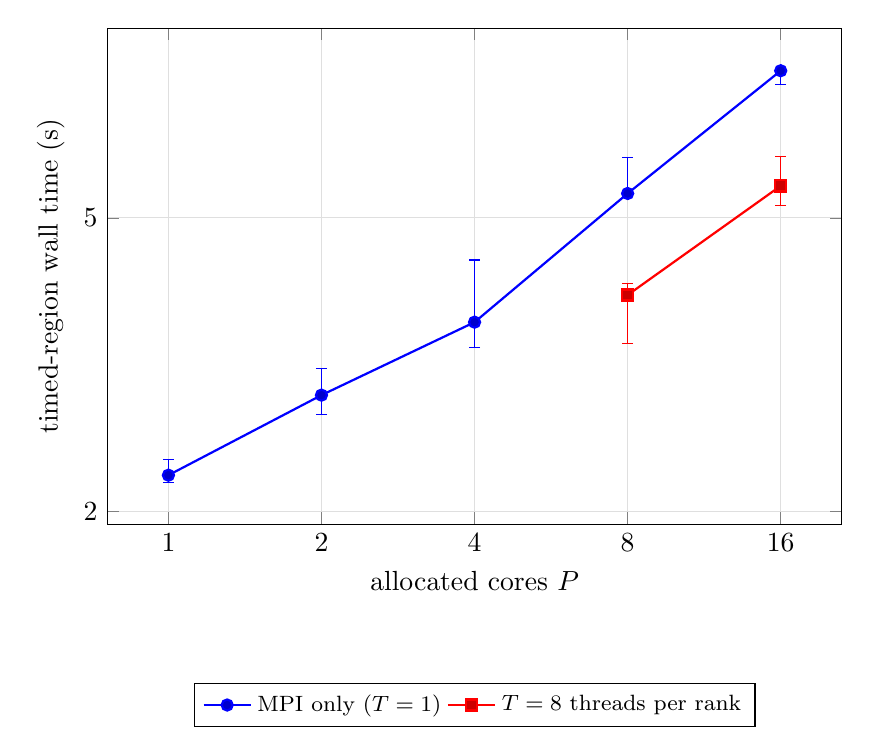
\begin{tikzpicture}
\begin{axis}[width=0.9\columnwidth, height=0.65\columnwidth, xlabel={allocated cores $P$}, ylabel={timed-region wall time (s)}, xmode=log, log basis x=2, log ticks with fixed point, ymode=log, ytick={1,2,5,10,20,50}, legend style={at={(0.5,-0.32)}, anchor=north, legend columns=2, font=\footnotesize}, legend cell align=left, grid=major, grid style={gray!25}]
\addplot+[mark=*, thick, error bars/.cd, y dir=both, y explicit] coordinates {(1,2.238) += (0,0.1127) -= (0,0.05345) (2,2.874) += (0,0.2539) -= (0,0.1693) (4,3.61) += (0,0.7735) -= (0,0.271) (8,5.396) += (0,0.6407) -= (0,0.01382) (16,7.919) += (0,0.02915) -= (0,0.329)};
\addlegendentry{MPI only ($T=1$)}
\addplot+[mark=square*, thick, error bars/.cd, y dir=both, y explicit] coordinates {(8,3.93) += (0,0.1425) -= (0,0.5505) (16,5.526) += (0,0.5307) -= (0,0.3289)};
\addlegendentry{$T=8$ threads per rank}
\end{axis}
\end{tikzpicture}
\caption{Weak-scaling runtime. $T=1$: $P_0=1$, $N_0=50000$, 50000 particles per core; $T=8$: $P_0=8$, $N_0=400000$, 50000 particles per core. Constant particles per core is not constant work per core. Bars: fastest to slowest repetition. Vanda job 1523703: 16 cores of a shared Gold 6438N node, 3 interleaved repetitions.}
\label{fig:weak-runtime}
\end{figure}
